\subsection{One-Sided Paired Comparison Test} \label{cohort-user-one-sided-comparison}
In this section, a paired-test is carried out to determine if a task
preceded by the same task is executed faster.  The tests show that for
cohort 1,2,3 there is a non-zero improvement but for cohort 4, the
test cannot reject that there is no improvement.

The method does not try to test for confounders \ref{ref:confounding}  which are possible factors affecting both the decision of scheduling one task after another and the output which is duration. In this study, we try to account for the user and the cohort, but we are not able to control for day of the week, pet or part number which might be in the set of confounders. Confounders can change the analysis result significantly.
A similar approach in \ref{ref:grouping-similar-work} points out that there is statistical reason to believe that controlling for cohort and user still may not eliminate the effect of confounders.

\subsubsection{Purpose and method}
This analysis compares Same Cohort and Different Cohort DUR work time within
users, separately for Cohorts 1--4. Task durations are first averaged within
each user, cohort, and allocation pattern. Only users with both allocation
patterns in the same cohort are retained, so the comparison is paired by user.

The paired test is a one-sided paired $t$-test. The null hypothesis is that
Same Cohort is not faster than Different Cohort
($\text{Same Cohort}-\text{Different Cohort}\geq 0$); the alternative is
that this difference is less than zero, with $\alpha=0.05$. The density
plots in Figures~\ref{fig:cohort-user-one-sided-1}--\ref{fig:cohort-user-one-sided-4}
show the two distributions of user-level means on a base-10 logarithmic
horizontal axis.

The 95\% two-sided confidence intervals for each allocation-pattern mean and
the paired mean difference use Student's $t$ distribution and the matched
users as the units of analysis. The one-sided 95\% upper bounds correspond to
the directional paired tests.

The source query keeps transitions on or after 2026-08-01, DUR tasks with
final status \texttt{CLOSED}, non-null user and start time, work time between
0.01 and 5 minutes, and known item cohorts. Rows without a previous cohort
are excluded.

\subsubsection{User-level work-time densities}
\begin{center}
\begin{minipage}{\linewidth}
\centering
\begin{minipage}[t]{0.49\linewidth}
\vspace{0pt}\centering
\fbox{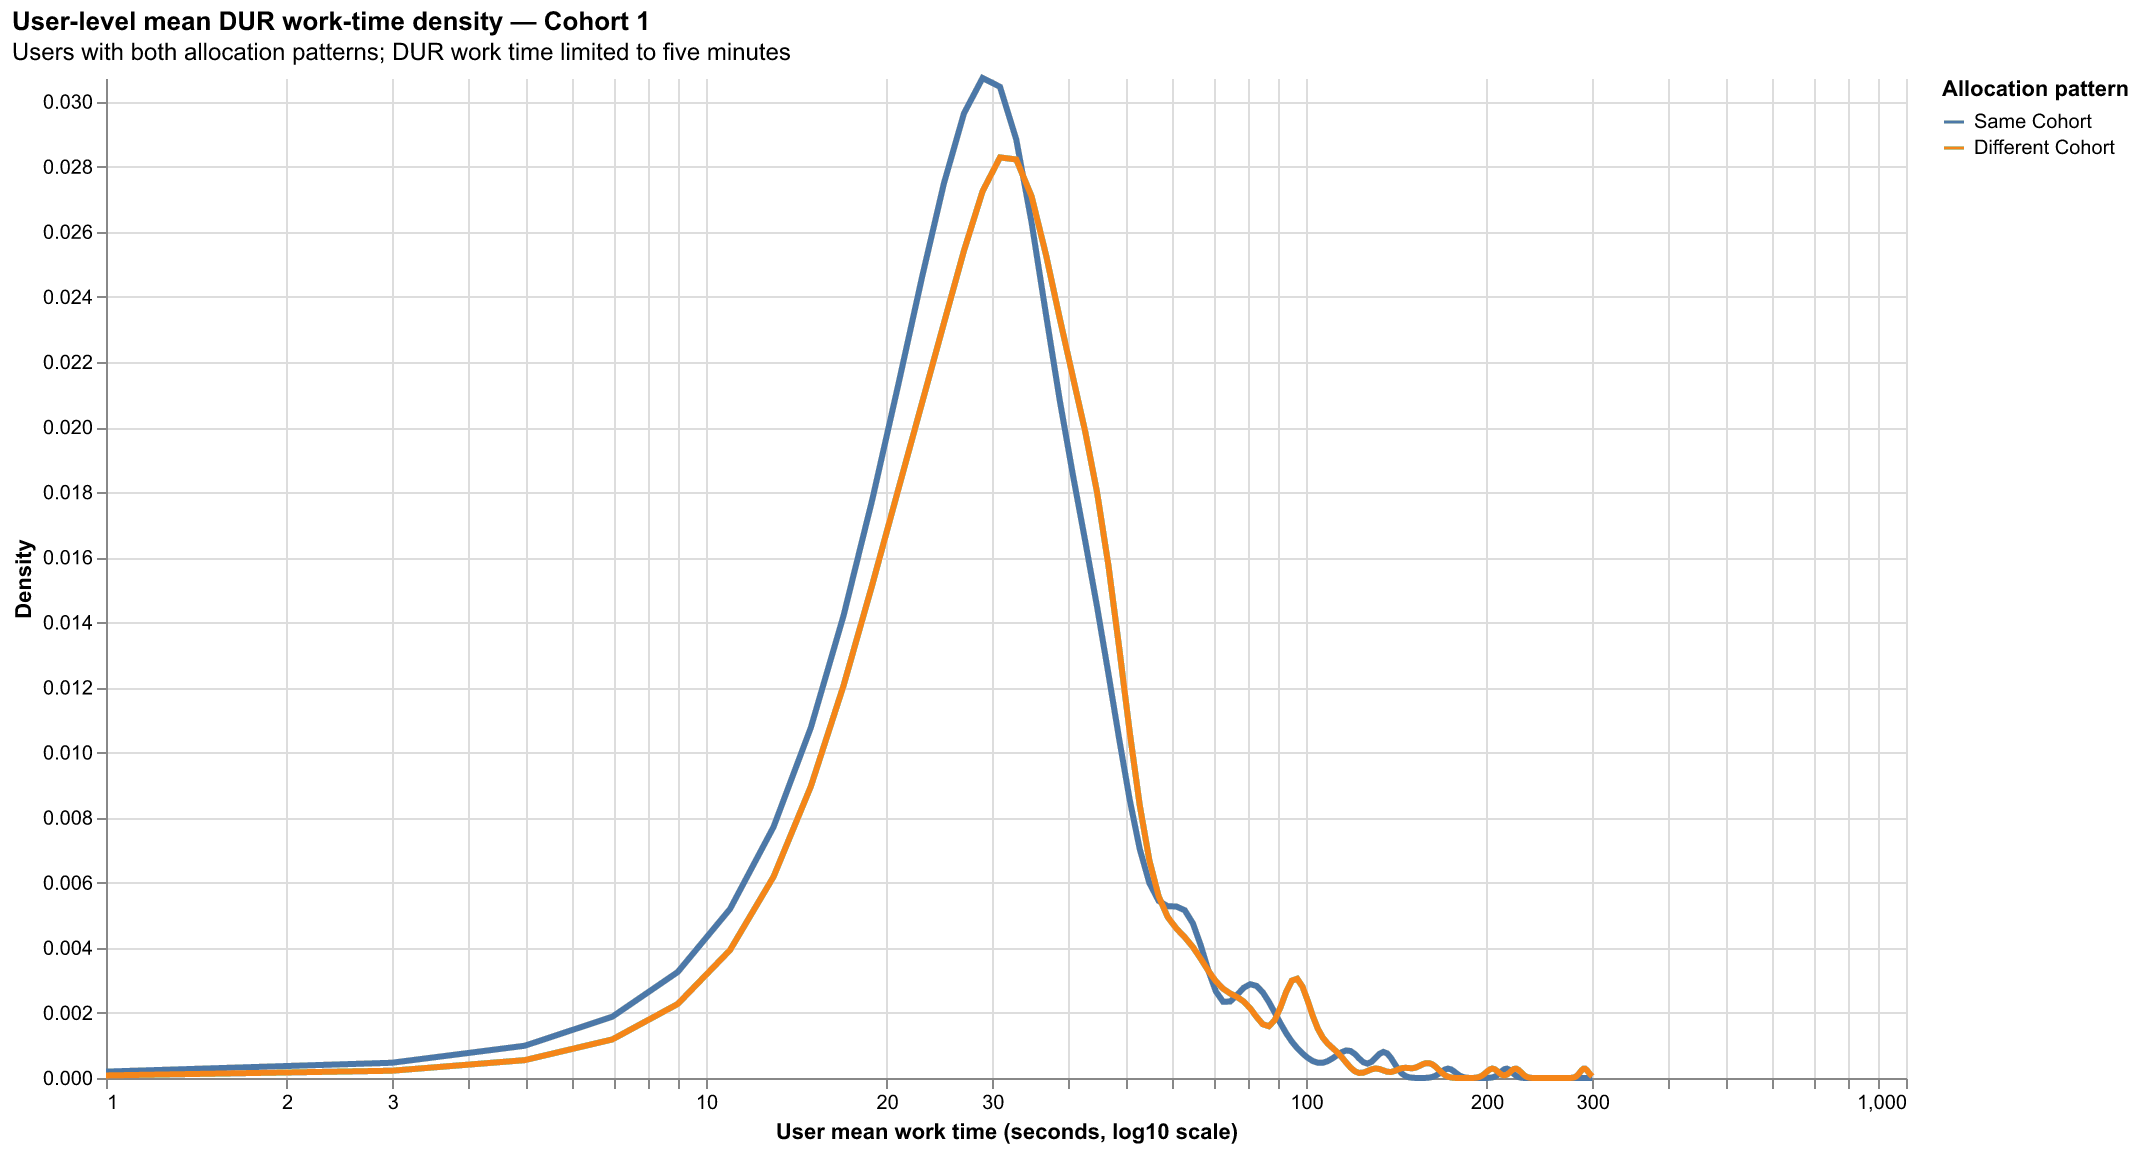
\includegraphics[width=\dimexpr\linewidth-2\fboxsep-2\fboxrule\relax,keepaspectratio,alt={User-level work-time density for Cohort 1}]{outputs/charts/stats-comparison-user/stats-comparison-user-cohort-1.png}}
\captionof{figure}{User-level work-time density, Cohort 1.}\label{fig:cohort-user-one-sided-1}
\end{minipage}\hfill
\begin{minipage}[t]{0.49\linewidth}
\vspace{0pt}\centering
\fbox{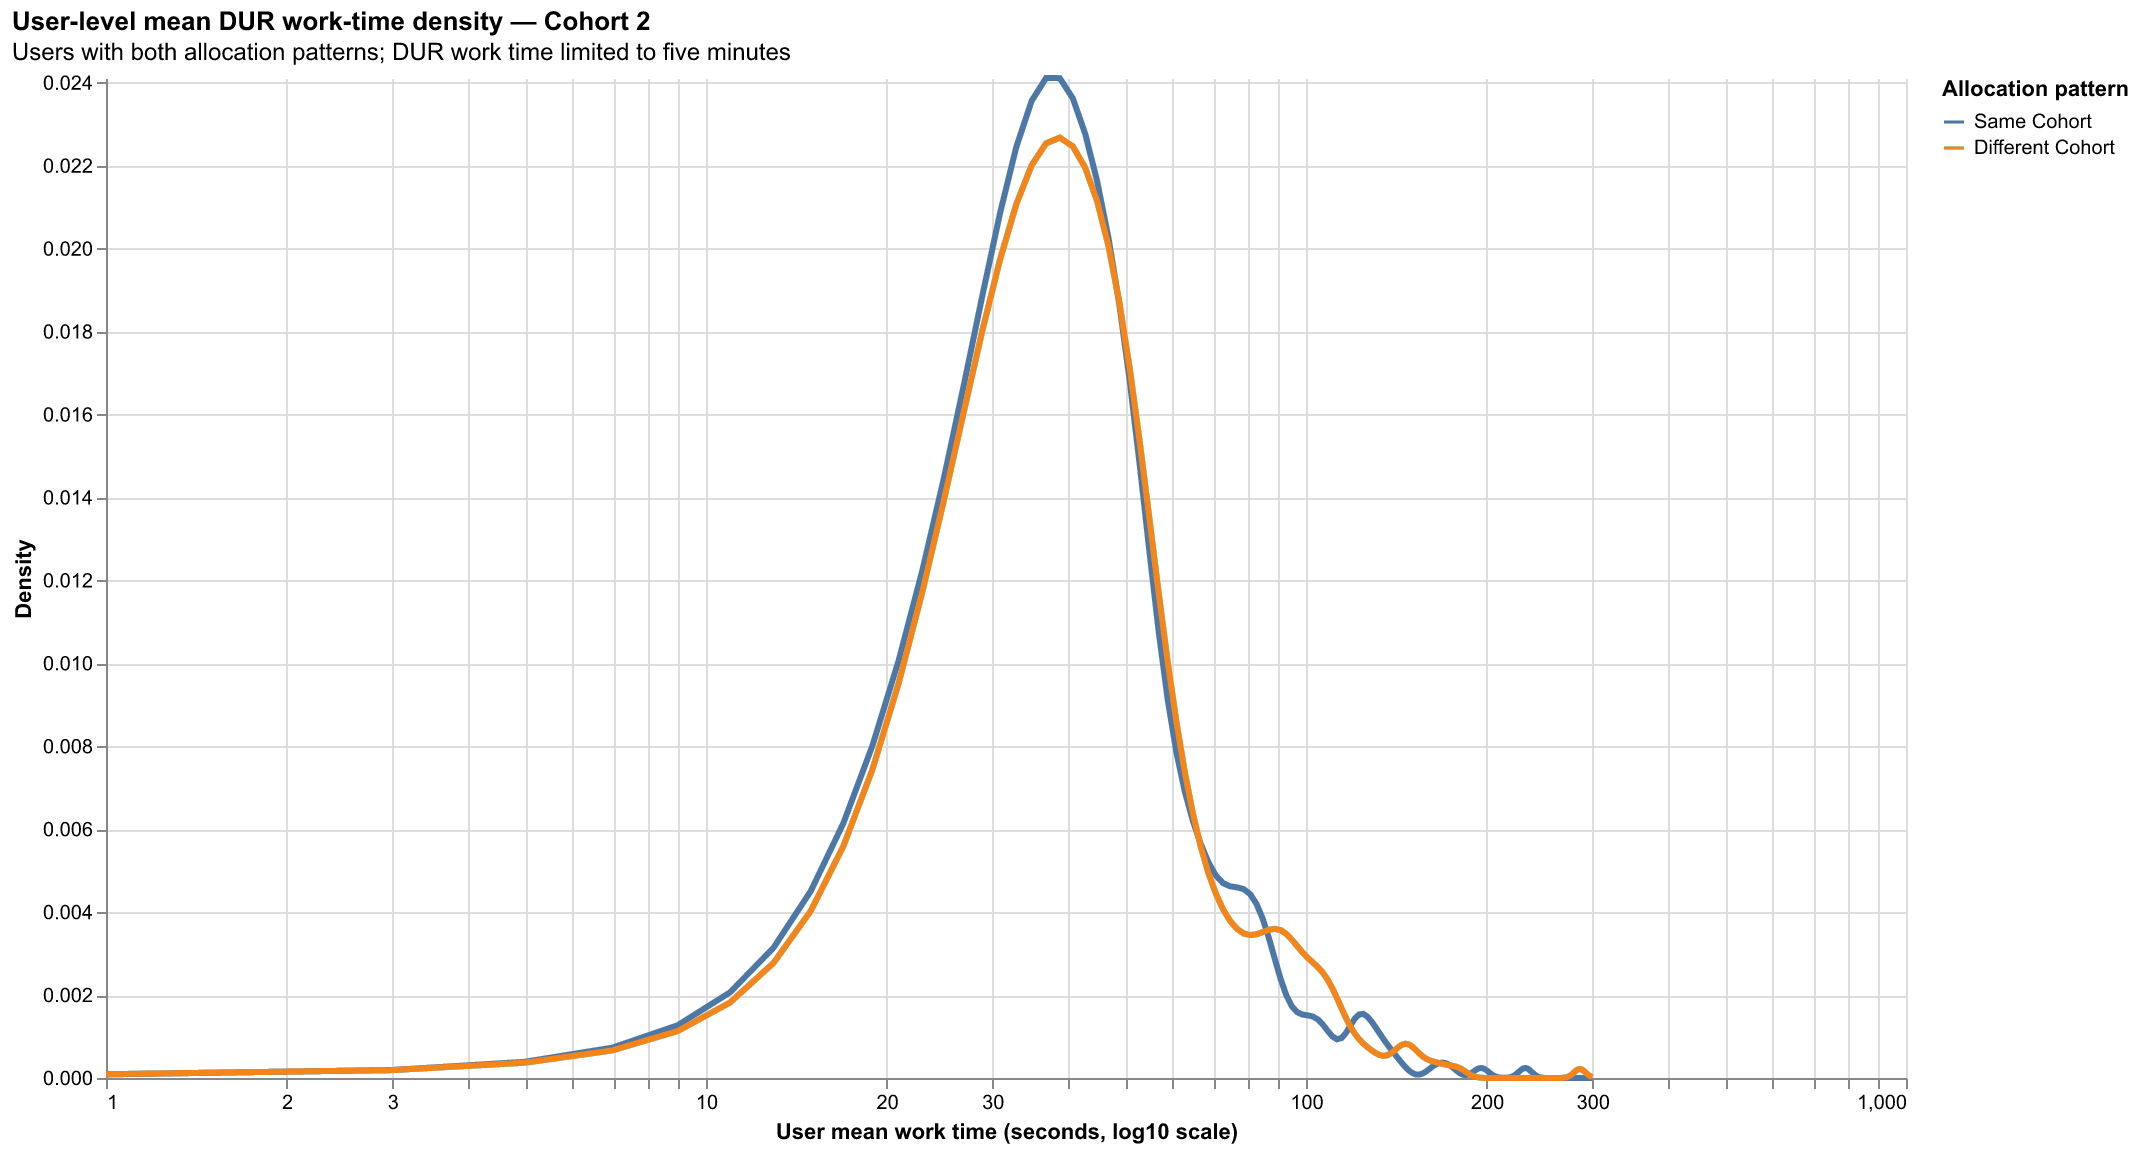
\includegraphics[width=\dimexpr\linewidth-2\fboxsep-2\fboxrule\relax,keepaspectratio,alt={User-level work-time density for Cohort 2}]{outputs/charts/stats-comparison-user/stats-comparison-user-cohort-2.png}}
\captionof{figure}{User-level work-time density, Cohort 2.}\label{fig:cohort-user-one-sided-2}
\end{minipage}

\vspace{0.7em}
\begin{minipage}[t]{0.49\linewidth}
\vspace{0pt}\centering
\fbox{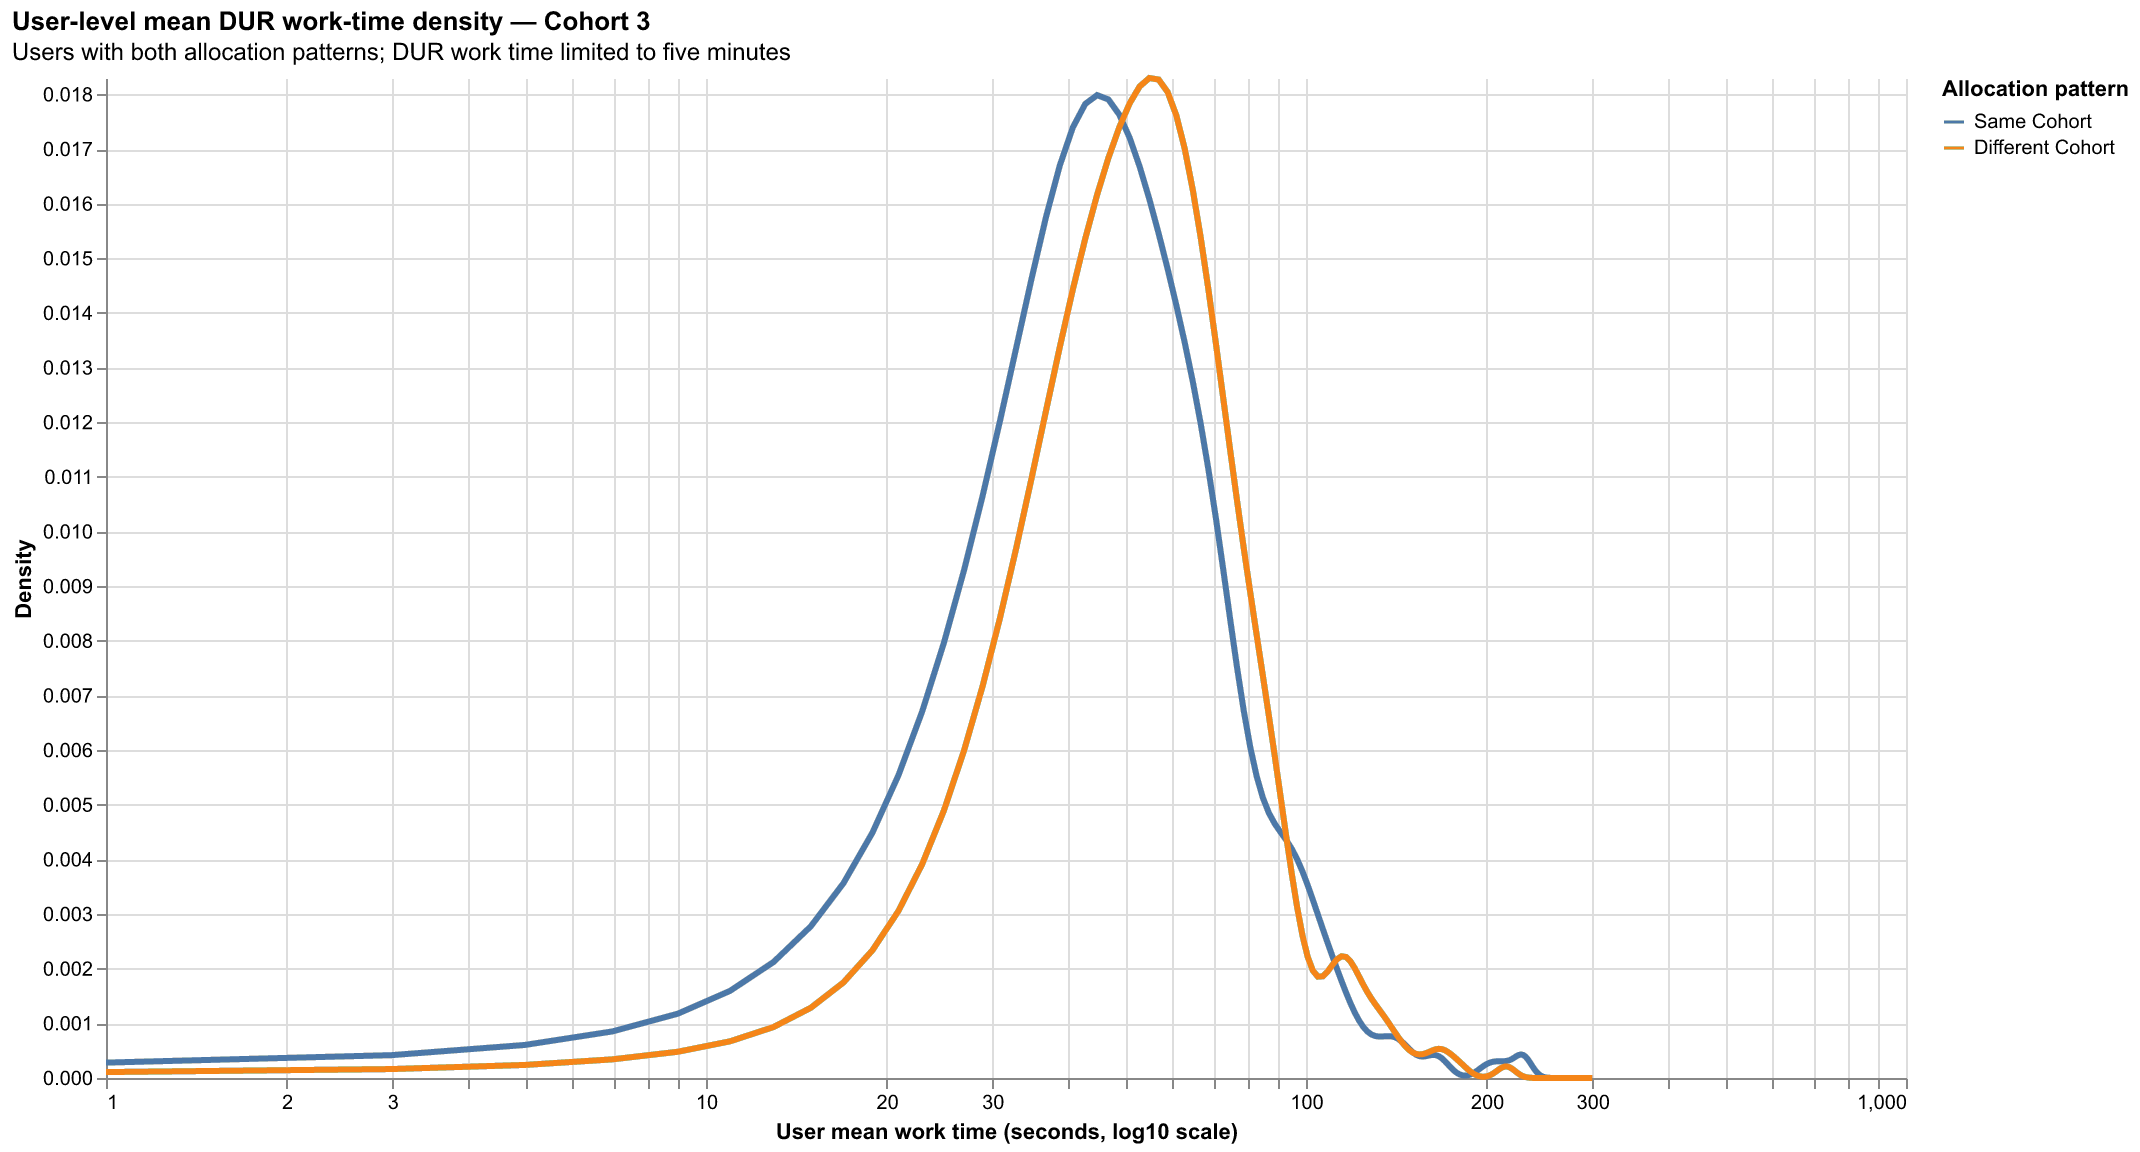
\includegraphics[width=\dimexpr\linewidth-2\fboxsep-2\fboxrule\relax,keepaspectratio,alt={User-level work-time density for Cohort 3}]{outputs/charts/stats-comparison-user/stats-comparison-user-cohort-3.png}}
\captionof{figure}{User-level work-time density, Cohort 3.}\label{fig:cohort-user-one-sided-3}
\end{minipage}\hfill
\begin{minipage}[t]{0.49\linewidth}
\vspace{0pt}\centering
\fbox{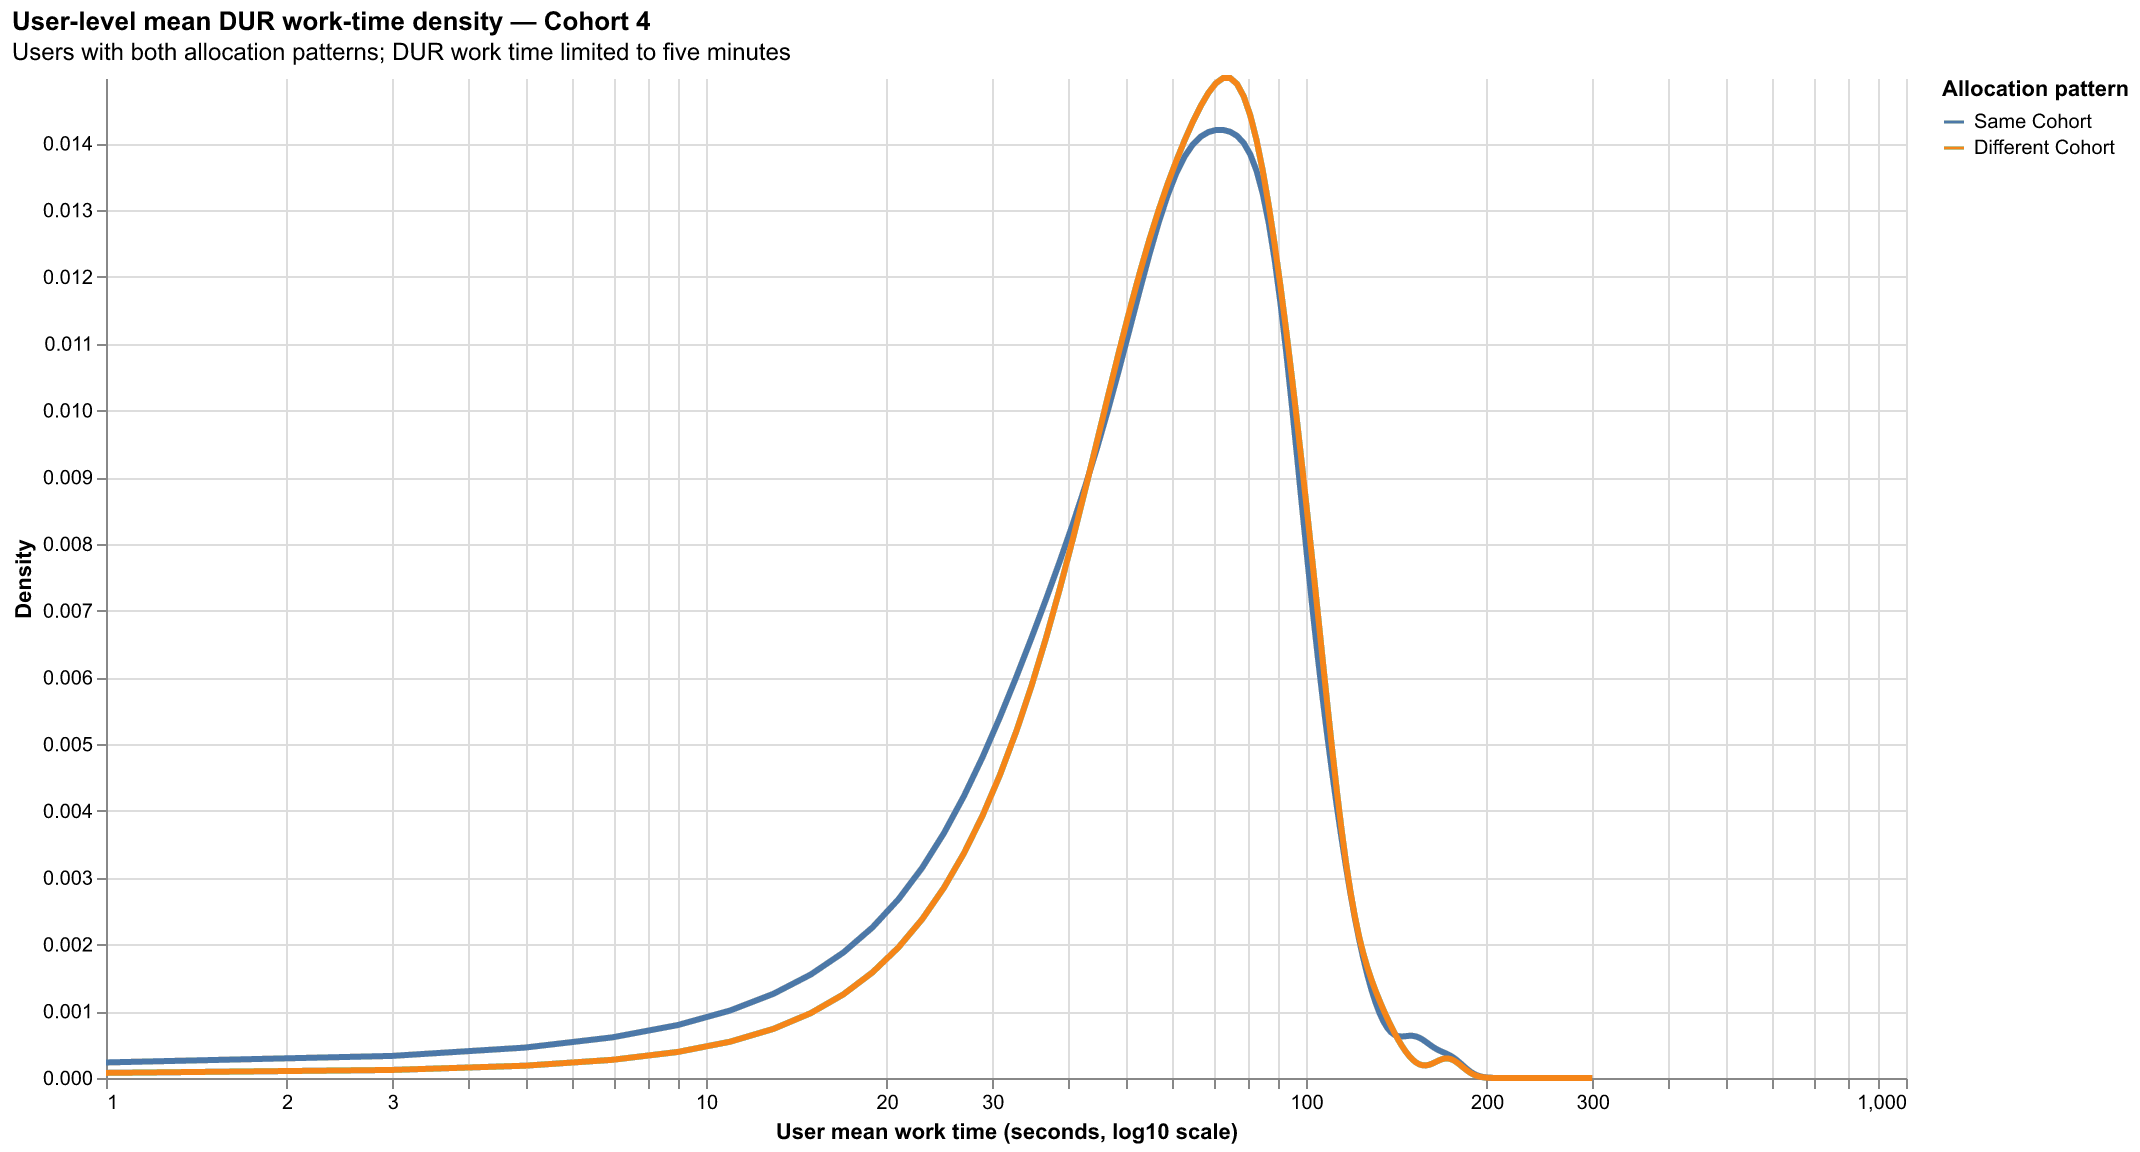
\includegraphics[width=\dimexpr\linewidth-2\fboxsep-2\fboxrule\relax,keepaspectratio,alt={User-level work-time density for Cohort 4}]{outputs/charts/stats-comparison-user/stats-comparison-user-cohort-4.png}}
\captionof{figure}{User-level work-time density, Cohort 4.}\label{fig:cohort-user-one-sided-4}
\end{minipage}
\end{minipage}
\end{center}

\subsubsection{Cohort results}
Table~\ref{tab:cohort-user-pattern-summary} reports the distribution of
user-level mean work times. The same matched users contribute to both rows
for each cohort.

\begin{center}
\begin{minipage}{\linewidth}
\centering\fontsize{8}{10}\selectfont
\begin{tabular}{@{}llrrlrrrr@{}}
\toprule
Cohort & Allocation pattern & Users & \shortstack{Mean user\\mean (min)} & \shortstack{95\% CI for mean\\(min)} & SD & Median & P25 & P75 \\
\midrule
1 & Same Cohort      & 289 & 0.6681 & $[0.6193,0.7170]$ & 0.4217 & 0.5410 & 0.4329 & 0.7469 \\
1 & Different Cohort & 289 & 0.7308 & $[0.6703,0.7912]$ & 0.5220 & 0.5909 & 0.4648 & 0.7776 \\
2 & Same Cohort      & 286 & 0.8402 & $[0.7831,0.8974]$ & 0.4910 & 0.7114 & 0.5552 & 0.9312 \\
2 & Different Cohort & 286 & 0.8767 & $[0.8155,0.9380]$ & 0.5259 & 0.7445 & 0.5660 & 0.9848 \\
3 & Same Cohort      & 250 & 1.0091 & $[0.9399,1.0783]$ & 0.5552 & 0.8809 & 0.6676 & 1.1693 \\
3 & Different Cohort & 250 & 1.0650 & $[1.0054,1.1247]$ & 0.4785 & 0.9695 & 0.7510 & 1.2296 \\
4 & Same Cohort      & 139 & 1.2037 & $[1.1285,1.2790]$ & 0.4488 & 1.1814 & 0.9098 & 1.4688 \\
4 & Different Cohort & 139 & 1.2202 & $[1.1504,1.2899]$ & 0.4161 & 1.2020 & 0.9106 & 1.4989 \\
\bottomrule
\end{tabular}
\captionof{table}{User-level mean DUR work time by cohort and allocation pattern.}\label{tab:cohort-user-pattern-summary}
\end{minipage}
\end{center}

The paired comparison uses the within-user difference
$\text{Same Cohort}-\text{Different Cohort}$. Table~\ref{tab:cohort-user-paired-test}
gives the one-sided test results. At the 0.05 level, the null hypothesis is
rejected for Cohorts 1--3 but not for Cohort 4.

\begin{center}
\begin{minipage}{\linewidth}
\centering\fontsize{8}{10}\selectfont
\begin{tabular}{@{}rrrllrrl@{}}
\toprule
Cohort & Users & \shortstack{Mean difference\\(min)} & \shortstack{95\% two-sided CI\\(min)} & \shortstack{95\% one-sided\\upper bound} & $t$ & df & One-sided $p$ \\
\midrule
1 & 289 & $-0.0626$ & $[-0.0972,-0.0281]$ & $(-\infty,-0.0337]$ & $-3.5706$ & 288 & 0.000208592 \\
2 & 286 & $-0.0365$ & $[-0.0703,-0.0028]$ & $(-\infty,-0.0082]$ & $-2.1302$ & 285 & 0.0170078 \\
3 & 250 & $-0.0559$ & $[-0.1043,-0.0075]$ & $(-\infty,-0.0154]$ & $-2.2766$ & 249 & 0.0118295 \\
4 & 139 & $-0.0164$ & $[-0.0557,0.0229]$  & $(-\infty,0.0165]$  & $-0.8272$ & 138 & 0.204771 \\
\bottomrule
\end{tabular}
\captionof{table}{One-sided paired tests of Same Cohort minus Different Cohort mean work time.}\label{tab:cohort-user-paired-test}
\end{minipage}
\end{center}

\subsubsection{Data}
The data is obtained using the following query.

\begingroup\fontsize{8}{9}\selectfont
\begin{verbatim}
WITH ordered AS (
  SELECT
    TASK_ID, USER_ID, ITEM_COHORT, STARTED_AT,
    TRANSITION_STARTED_AT::DATE AS dt,
    LAG(ITEM_COHORT) OVER (
      PARTITION BY USER_ID, TRANSITION_STARTED_AT::DATE
      ORDER BY STARTED_AT
    ) AS prev_cohort,
    DWELL_IN_PROGRESS_TO_CLOSED_MINUTES AS work_min
  FROM EDLDB.PET_HEALTH_ANALYTICS_SANDBOX.FCT__TASKS_LIFECYCLE
  WHERE TRANSITION_STARTED_AT >= '2026-08-01'
    AND TASK_TYPE = 'DUR' AND FINAL_STATUS = 'CLOSED'
    AND USER_ID IS NOT NULL AND STARTED_AT IS NOT NULL
    AND DWELL_IN_PROGRESS_TO_CLOSED_MINUTES BETWEEN 0.01 AND 5
    AND ITEM_COHORT != 'Unknown'
)
SELECT
  TASK_ID AS task_id, USER_ID AS user_id, dt,
  CASE
    WHEN ITEM_COHORT = prev_cohort THEN 'Same Cohort'
    ELSE 'Different Cohort'
  END AS allocation_pattern,
  ITEM_COHORT AS cohort, work_min
FROM ordered
WHERE prev_cohort IS NOT NULL
ORDER BY allocation_pattern, work_min
\end{verbatim}
\endgroup
